%% GENERATED by tools/from_docs.py from stepss-docs. Do not edit by hand:
%% edit the page named below in stepss-docs and regenerate.
%% source: stepss-docs/src/content/docs/gui/interface.mdx

\chapter{The STEPSS GUI interface}\label{doc:gui-interface}

The window is six tabs, and you use them roughly left to right: name the files,
choose what to record, solve the initial operating point, run the simulation,
then analyse the result. The sixth builds your own models.

This page says what each tab is for. It does not describe the file formats
themselves; \hyperref[ch-files]{File Formats} and
\hyperref[ch-sync]{Dynamic Data Records} own those.

\section{System Data}\label{gui-interface:system-data}

Where the case is named. Nine numbered rows take the \textbf{system data files}, and a
separate row below takes the \textbf{disturbance file}. Both groups are required.

Each row has a \textbf{Load file} button and a pencil that opens the file in an
editor. \textbf{Clear files} empties the tab.

\begin{figure}[htbp]
\centering
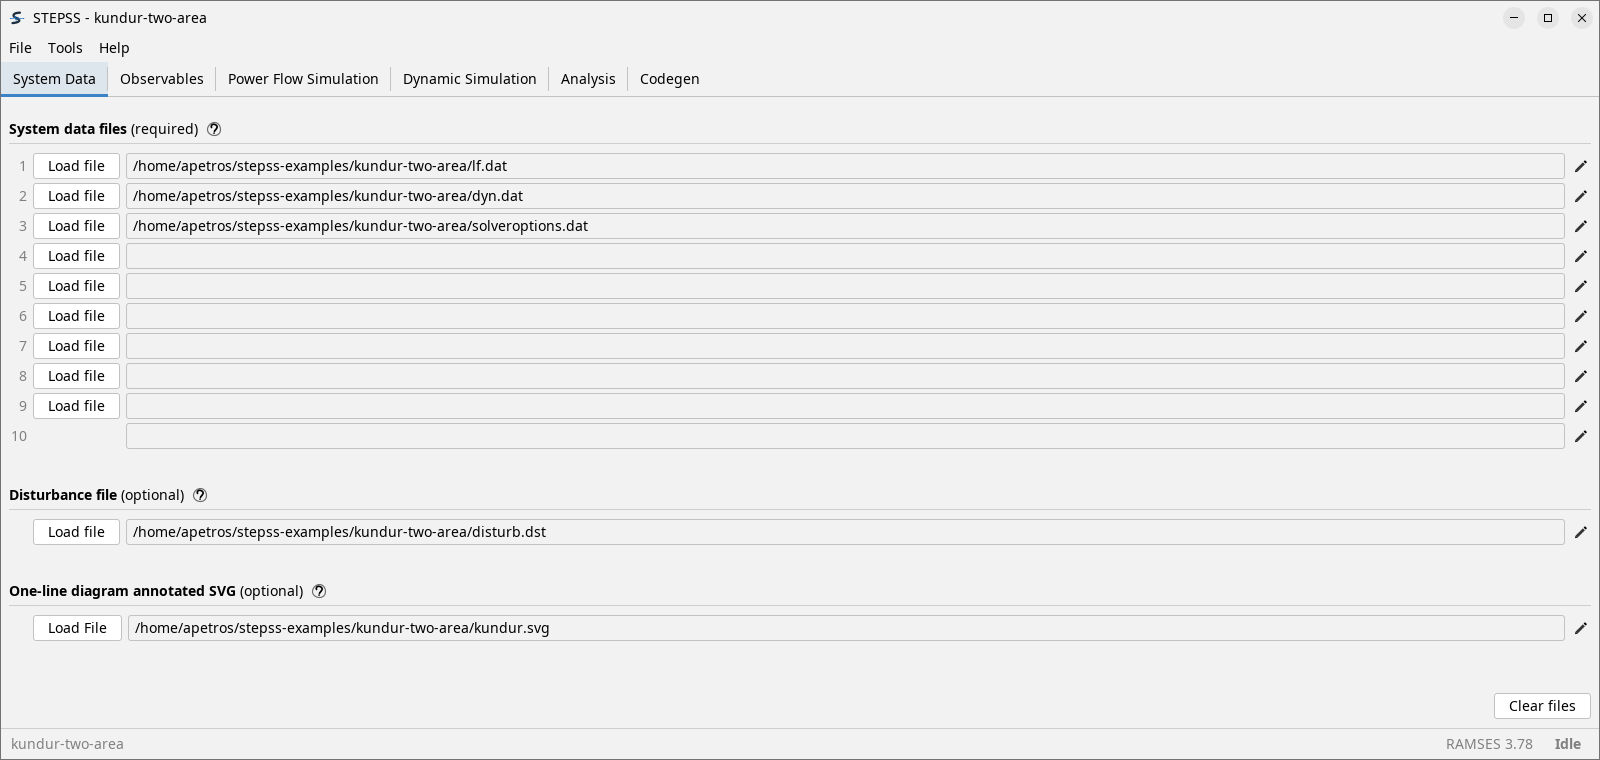
\includegraphics[width=0.98\linewidth]{figures/gui-system-data-light}
\caption{The System Data tab with the Kundur two-area case loaded.}
\end{figure}

Order does not matter and the rows need not be filled contiguously. Which files a
case needs depends on the study: a network description, dynamic component data
and solver settings are the usual three.

The last row takes an \textbf{annotated SVG one-line diagram}, a drawing of the
network with placeholder codes typed into it. Every \textbf{Run power flow} fills
those codes in with the solved values and opens the result in a window of its
own;
\hyperref[ch-pf]{Annotated One-line Diagram}
owns the codes and the authoring.

\section{Observables}\label{gui-interface:observables}

Two separate jobs share this tab: what you watch \textbf{while} the simulation runs,
and what gets written to disk for afterwards.

\subsection{Runtime observables}\label{gui-interface:runtime-observables}

Three rows, each pairing a quantity with the name of the equipment to watch. Fill
any of them in and STEPSS plots those quantities live as the simulation advances.

The quantities on offer are bus voltage, machine speed, omega-delta and active
power-delta of a machine, centre of inertia, wall time, latency, branch active and
reactive power at either end, and an injector observable. The name beside it is the
equipment's own: a bus name for a bus voltage, a synchronous machine name for a
speed or a centre of inertia, and \texttt{RT} for wall time, which plots wall clock
against simulation time.

\begin{figure}[htbp]
\centering
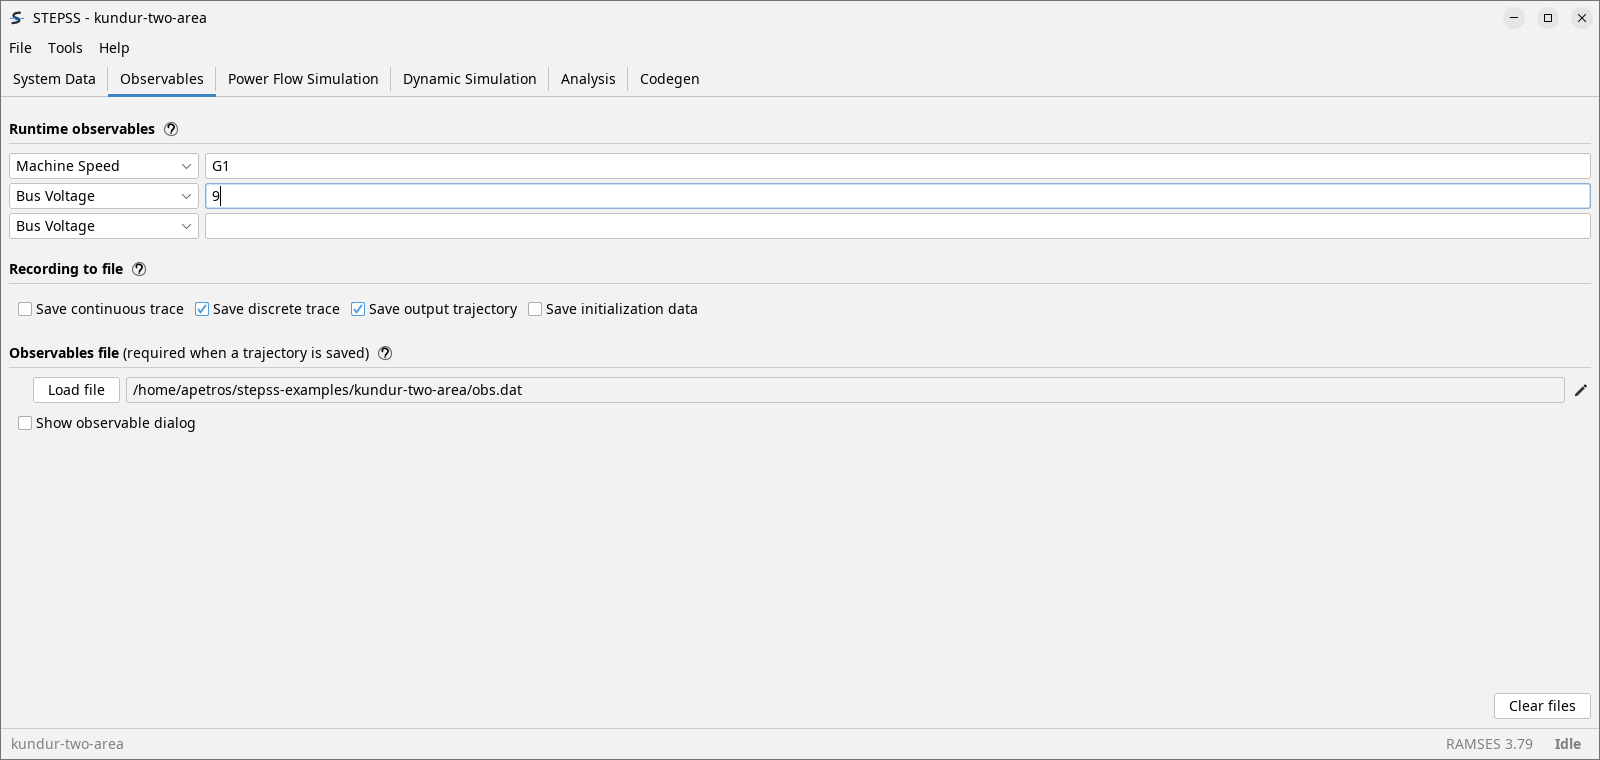
\includegraphics[width=0.98\linewidth]{figures/gui-observables-light}
\caption{The Observables tab.}
\end{figure}

A quantity may be followed by extra gnuplot commands, separated by \texttt{/}. They are
passed through into the \texttt{.plt} script the engine writes, for anyone who opens
that file in gnuplot. They have no effect on the curves STEPSS draws.

Live plotting needs nothing installed; see
\hyperref[doc:gui-first-run]{First Run}.

\subsection{Recording to file}\label{gui-interface:recording-to-file}

Four independent choices, on one row: save the \textbf{continuous trace}, the
\textbf{discrete trace}, the \textbf{output trajectory}, and the \textbf{initialization data}.
The last of those writes the settings, the comments and the initialization data
to \texttt{dump.trace}; hover any of the four for what it records.

The \textbf{observables file} below them is required whenever a trajectory is saved,
because it is what says which quantities the trajectory should contain.
\hyperref[ch-files]{Observables File} gives its syntax
and the eight equipment types it accepts. \textbf{Show observable dialog} builds one
interactively instead of writing it by hand.

Ticking it opens eight rows under the tab, one per equipment type. Name a piece
of equipment and \textbf{Add} puts it on that row's list, \textbf{All} takes every one of
that type in the case, and the list beside it is what will be recorded.

\begin{figure}[htbp]
\centering
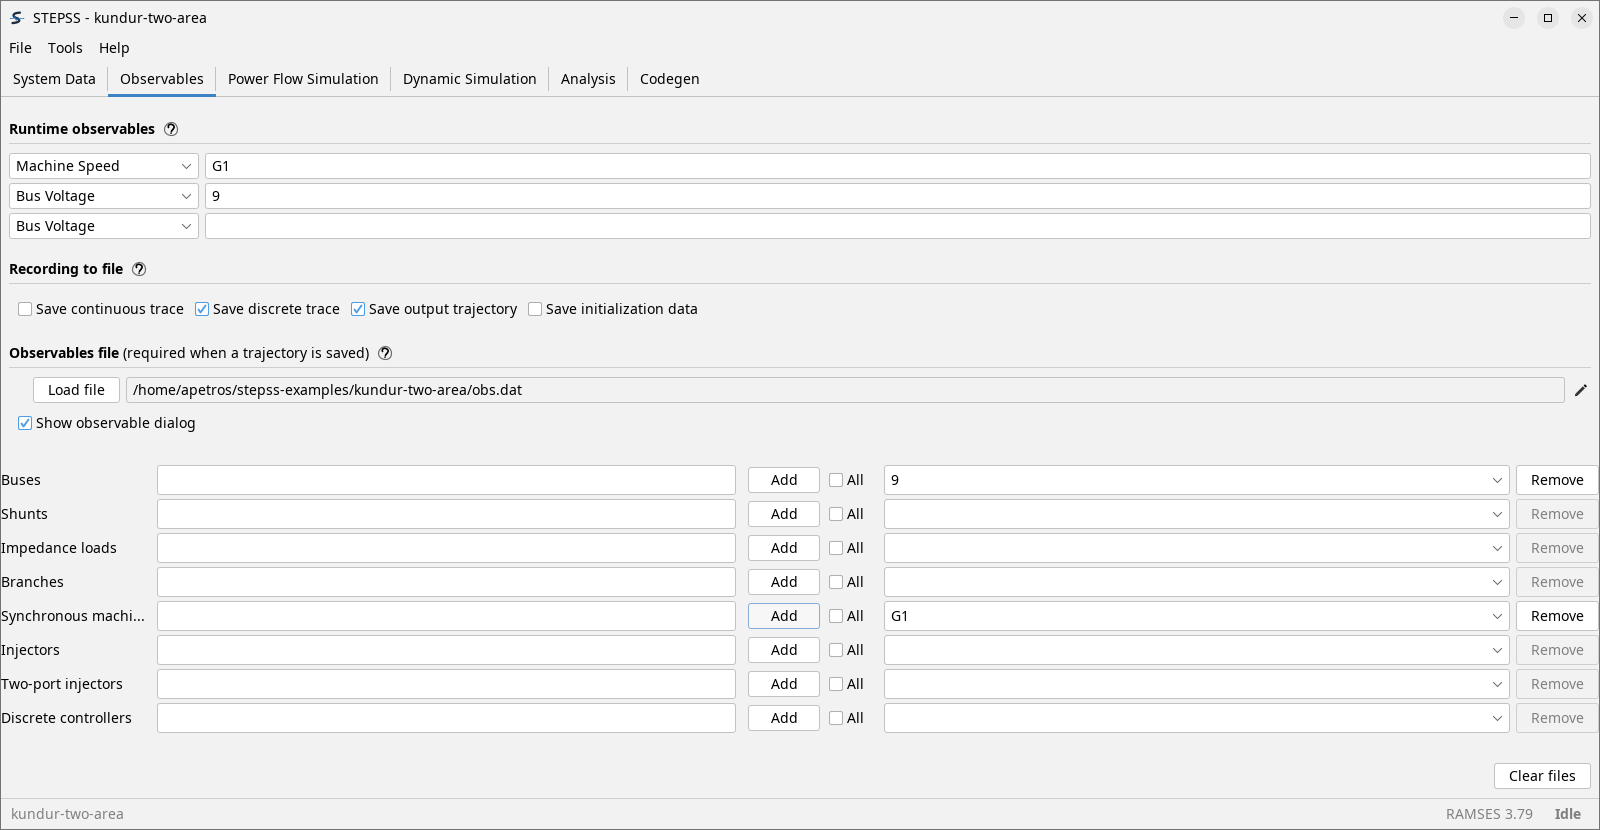
\includegraphics[width=0.98\linewidth]{figures/gui-observable-picker-light}
\caption{The Observables tab with Show observable dialog ticked.}
\end{figure}

The eight lists are session state and are not written into a saved
configuration, so a case saved with the box ticked comes back needing them
filled in again.

\section{Power Flow Simulation}\label{gui-interface:power-flow-simulation}

Where the power flow is solved, giving the operating point the dynamic simulation
starts from.

\textbf{Run power flow} calls \hyperref[ch-pf]{Helios} and reports into the
pane above: bus voltages and angles, the generator table with its limits, the
system power balance, and the files it exported.

Seven buttons enable once a run succeeds:

\begin{small}\begin{longtable}[]{@{}
  >{\raggedright\arraybackslash}p{(\linewidth - 4\tabcolsep) * \real{0.3663}}
  >{\raggedright\arraybackslash}p{(\linewidth - 4\tabcolsep) * \real{0.6337}}
@{}}
\toprule\noalign{}
\begin{minipage}[b]{\linewidth}\raggedright
Button
\end{minipage} & \begin{minipage}[b]{\linewidth}\raggedright
What it does
\end{minipage} \\
\midrule\noalign{}
\endhead
\bottomrule\noalign{}
\endlastfoot
\textbf{Add Helios results to data} & Puts the solved \texttt{in\_volt\_trfo.dat} into system data row ten, so the dynamic simulation starts from this operating point \\
\textbf{Save power flow solution} & Keeps a copy of that file, which the next run would otherwise overwrite \\
\textbf{Bus overview} & Bus voltages and angles \\
\textbf{Branch flows} & P and Q at each end, losses, and loading against rated MVA \\
\textbf{Generators \& SVCs} & Generator and SVC output, against their limits \\
\textbf{Adjustable transformers} & Transformer ratios, including any Helios adjusted \\
\textbf{Global power balance} & Generation, load, shunts and network losses \\
\end{longtable}\end{small}

\begin{figure}[htbp]
\centering
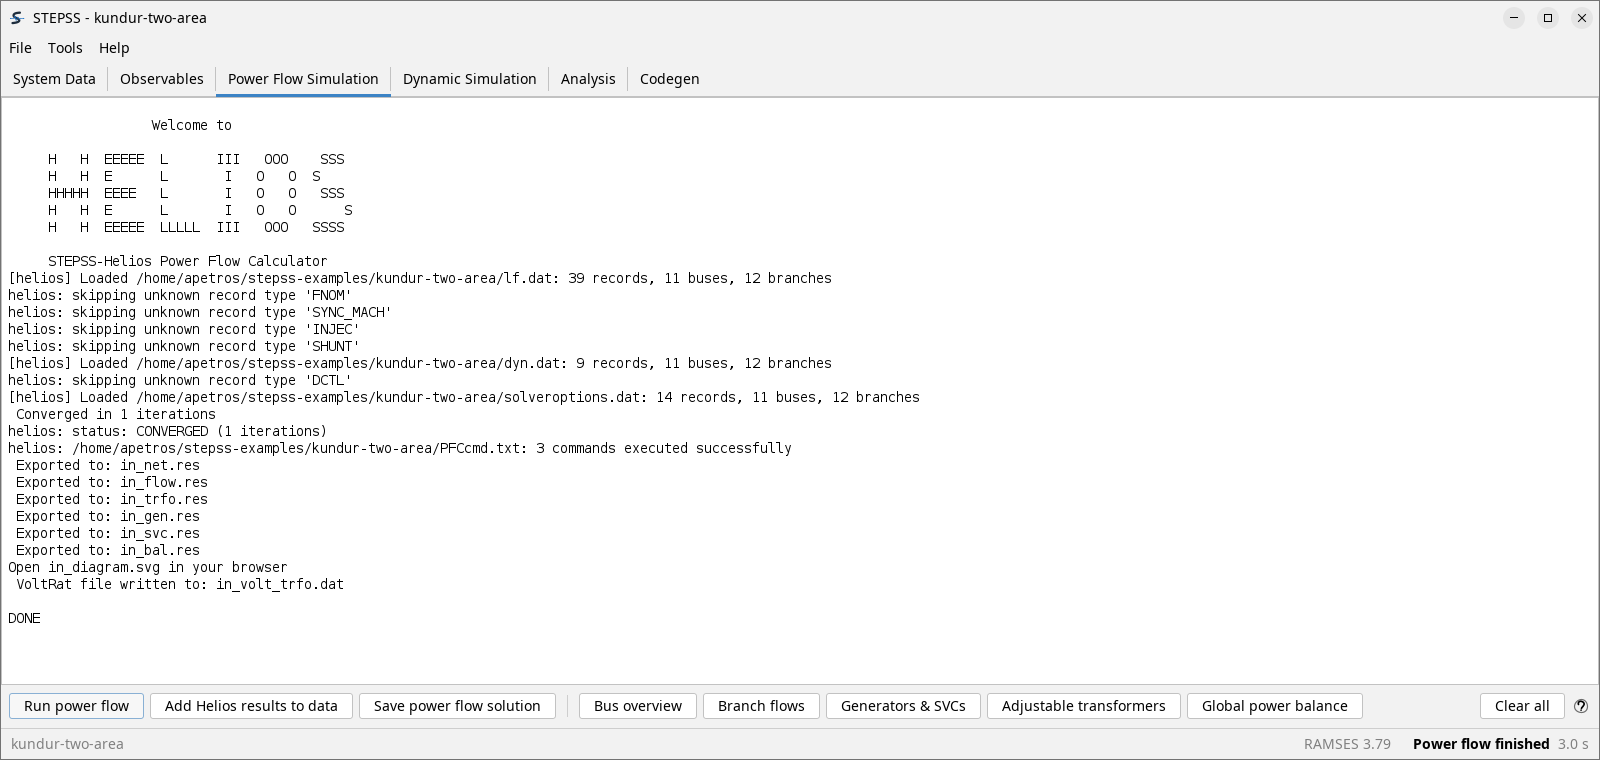
\includegraphics[width=0.98\linewidth]{figures/gui-power-flow-light}
\caption{The Power Flow Simulation tab after a successful run on the Kundur case.}
\end{figure}

Each of the four inspection buttons writes its table into the same pane, so the
run's log and the answer you asked for stay in one place.

\textbf{Bus overview}

\begin{figure}[htbp]
\centering
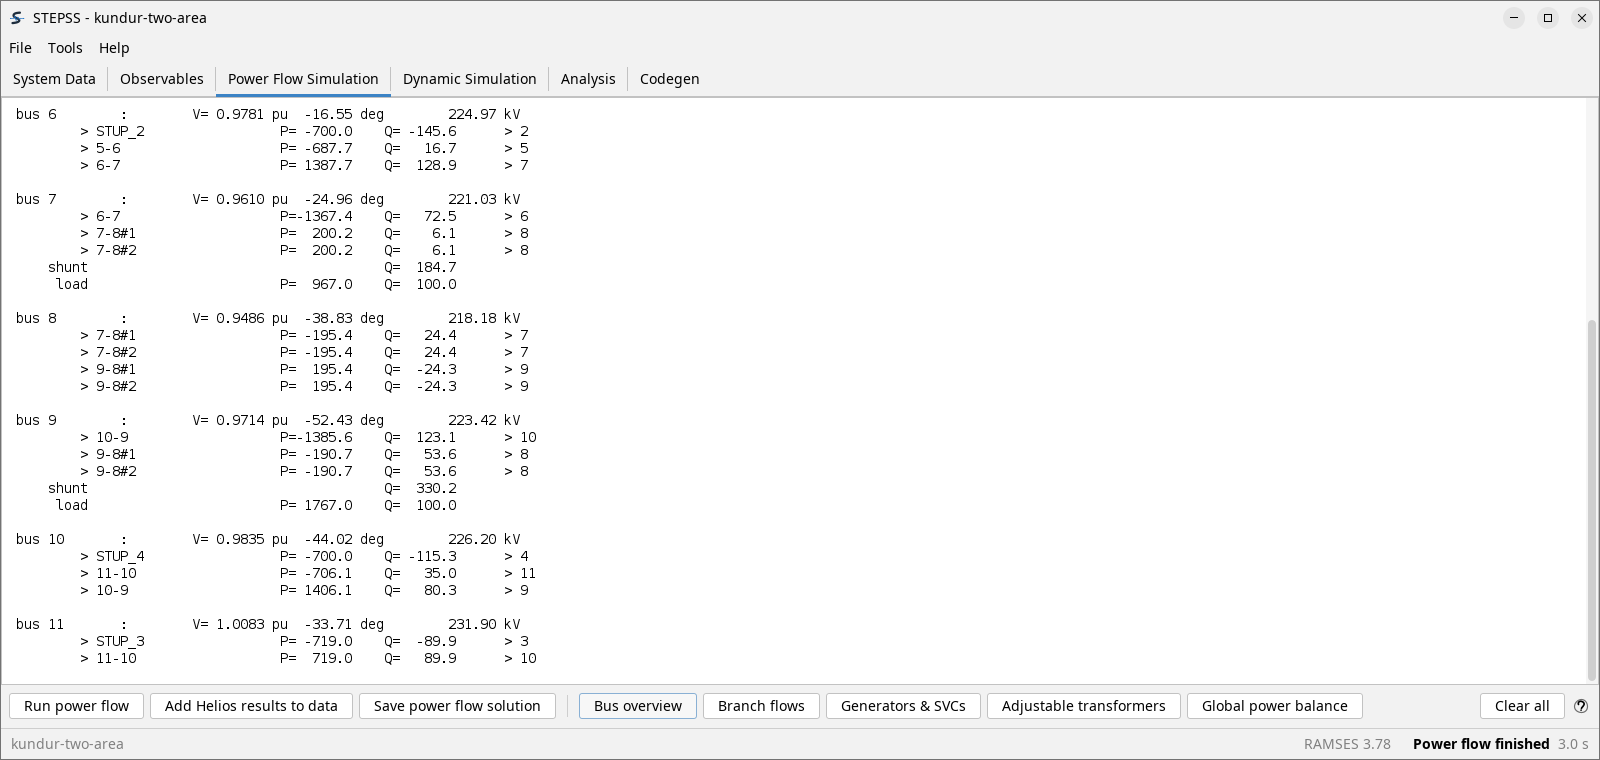
\includegraphics[width=0.98\linewidth]{figures/gui-bus-overview-light}
\caption{The Power Flow Simulation pane showing the bus overview for the Kundur case.}
\end{figure}

\textbf{Branch flows}

\begin{figure}[htbp]
\centering
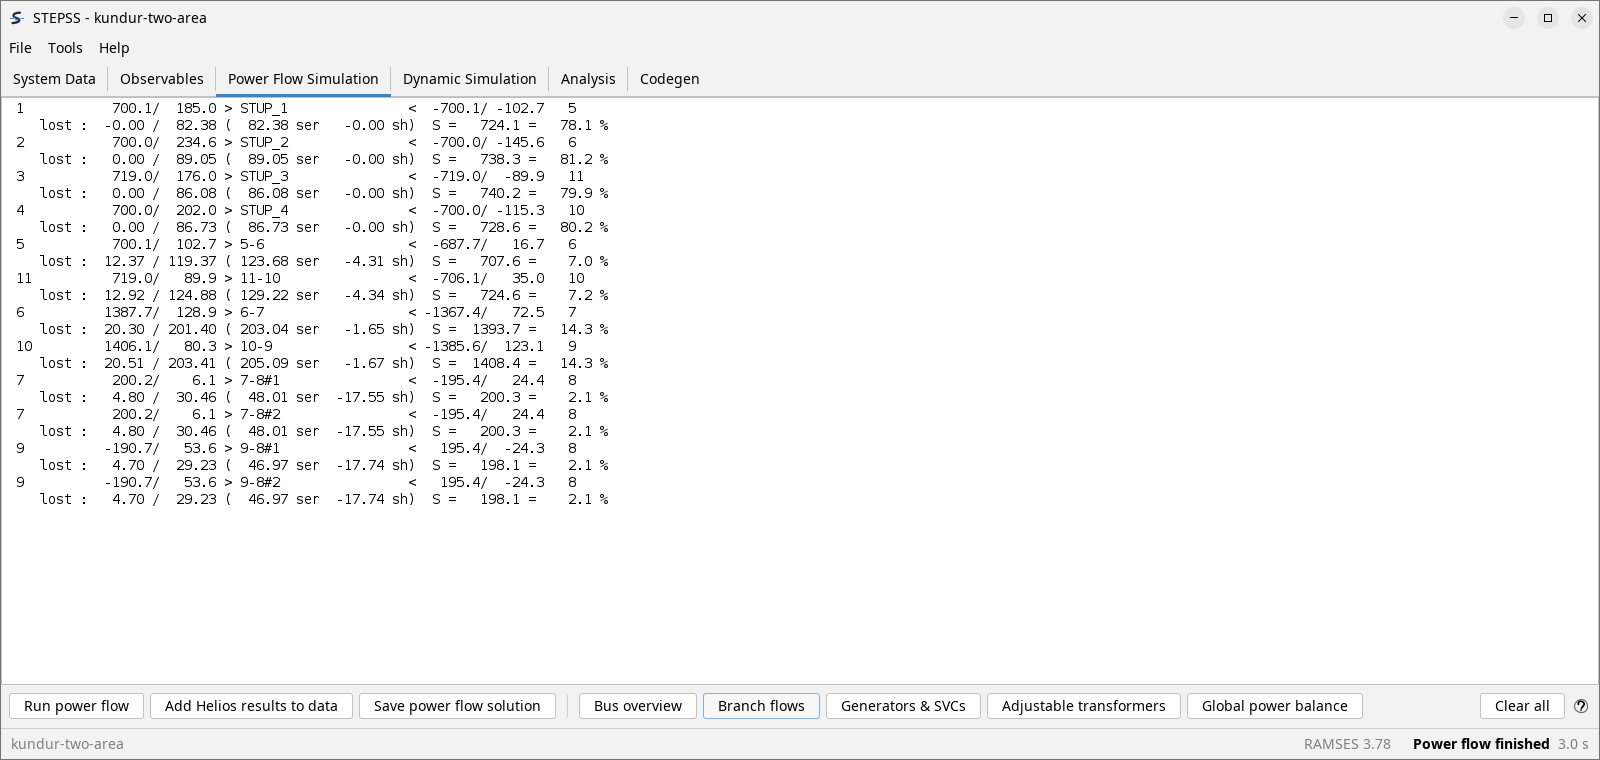
\includegraphics[width=0.98\linewidth]{figures/gui-branch-flows-light}
\caption{The Power Flow Simulation pane showing branch flows for the Kundur case.}
\end{figure}

\textbf{Generators \& SVCs}

\begin{figure}[htbp]
\centering
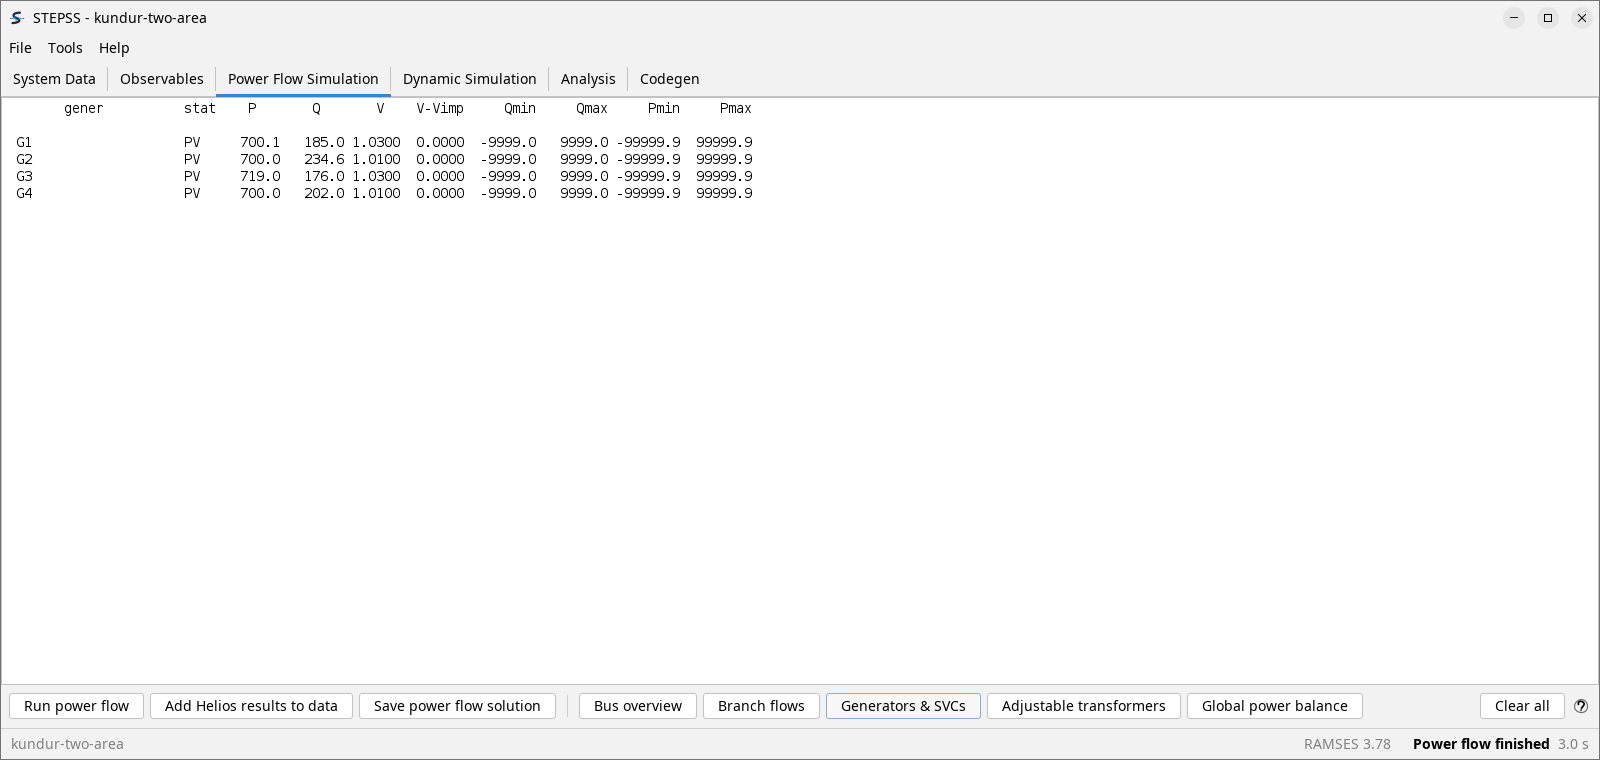
\includegraphics[width=0.98\linewidth]{figures/gui-generators-svcs-light}
\caption{The Power Flow Simulation pane showing the generator table for the Kundur case.}
\end{figure}

\textbf{Global power balance}

\begin{figure}[htbp]
\centering
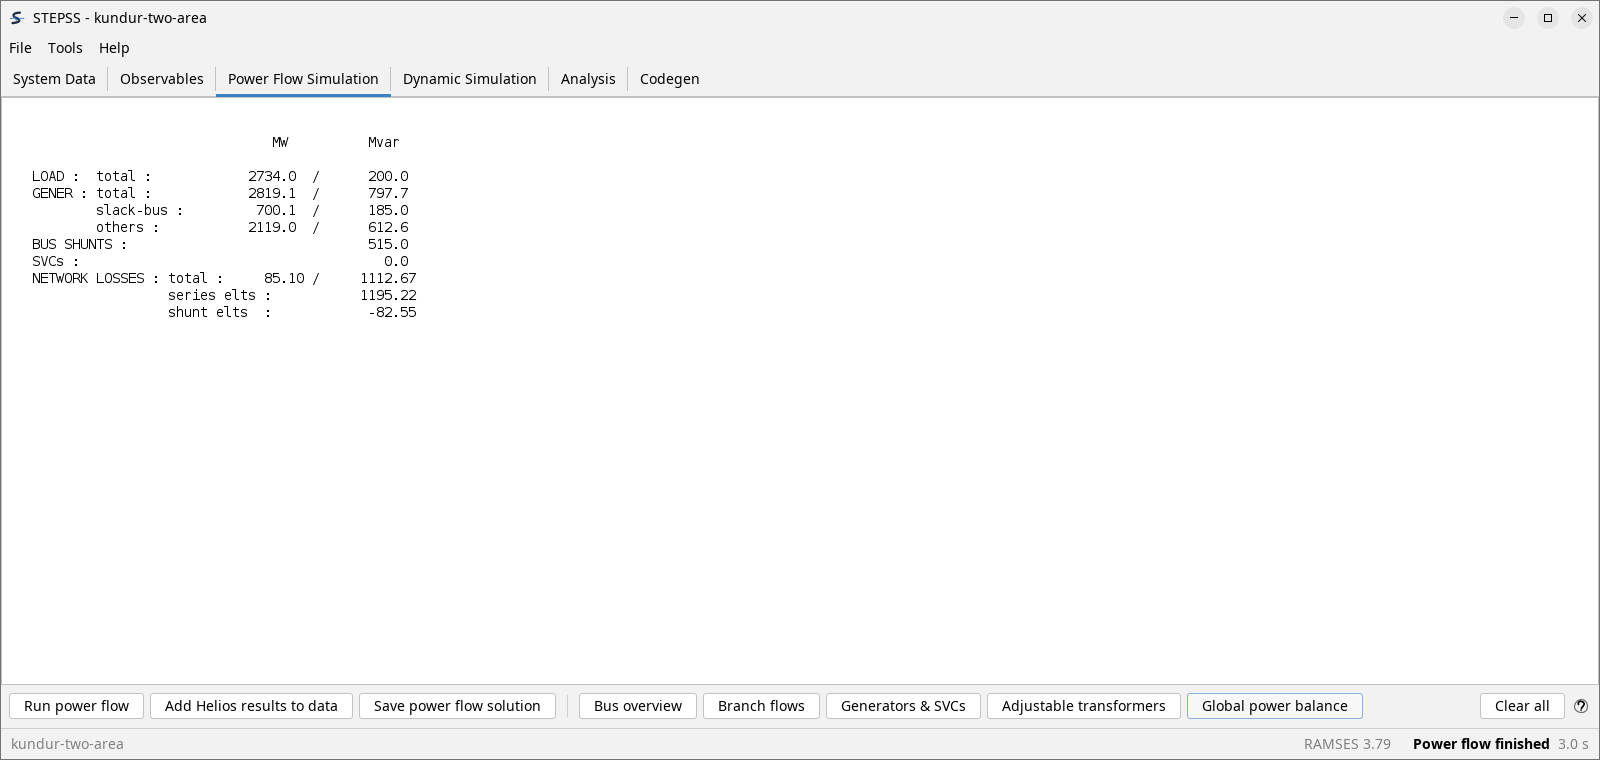
\includegraphics[width=0.98\linewidth]{figures/gui-power-balance-light}
\caption{The Power Flow Simulation pane showing the global power balance for the Kundur case, in MW and Mvar.}
\end{figure}

\textbf{Adjustable transformers} has no tab above it because the Kundur case has no
adjustable transformer to report; on a case that has them, it lists each one's
ratio and marks any that Helios moved.

A case that also loaded a one-line diagram gets a window of its own on every
run, with the solved values substituted into the drawing.

\begin{figure}[htbp]
\centering
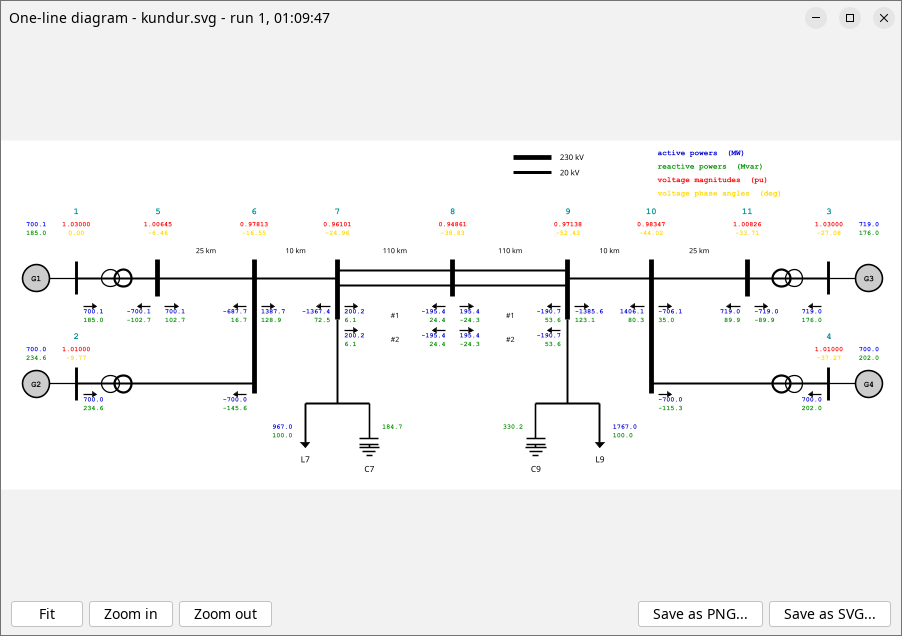
\includegraphics[width=0.98\linewidth]{figures/gui-one-line-diagram-light}
\caption{The one-line diagram window for the Kundur case, titled One-line diagram, kundur.svg, run 1.}
\end{figure}

\section{Dynamic Simulation}\label{gui-interface:dynamic-simulation}

Where the case is run. \textbf{Run dynamic simulation} starts
\hyperref[ch-overview]{RAMSES} and \textbf{Stop simulation} ends it
early.

The pane reports the settings in force, the integration method and tolerances,
whether parallelism is active, and on completion the elapsed time, the number of
time steps, and Jacobian, solution and evaluation counts for the network and the
injectors. Those counts are how you tell a cheap run from an expensive one.

The load buttons beside them read back a previous run's output, continuous trace,
discrete trace or initialization data, so a result can be examined without
re-running it. \textbf{Search} finds text in the pane.

\begin{figure}[htbp]
\centering
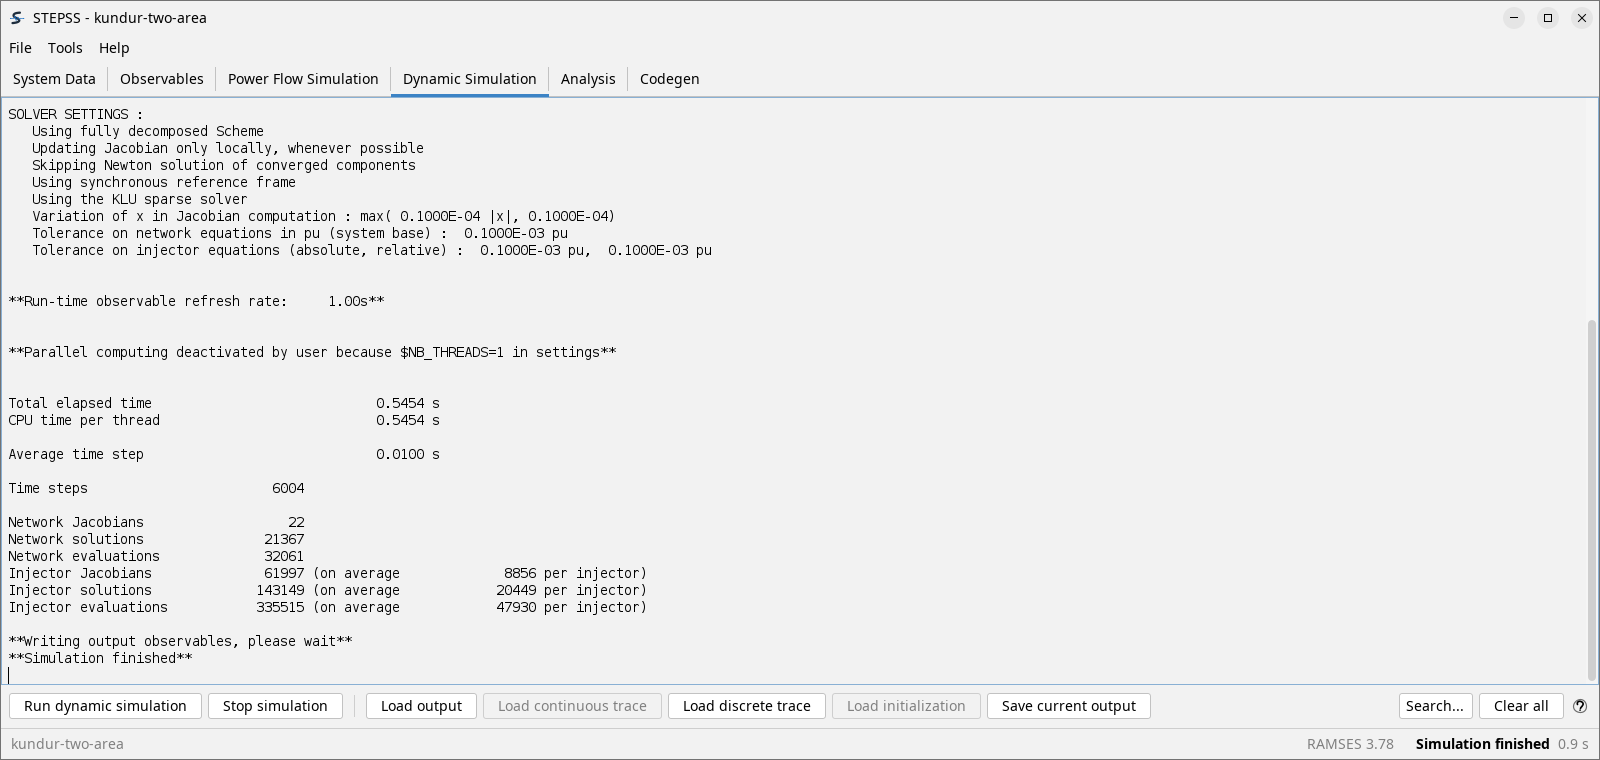
\includegraphics[width=0.98\linewidth]{figures/gui-dynamic-simulation-light}
\caption{The Dynamic Simulation tab after a completed run.}
\end{figure}

\section{Analysis}\label{gui-interface:analysis}

Two kinds of analysis, on the same solved case.

\textbf{Time-domain analysis} turns a saved trajectory into curves. \textbf{Extract curves}
opens a picker and then draws the result in a window of its own, one per
extraction, so two extractions can be compared side by side. Each window saves
its own figure as PNG, SVG or CSV, and its own \texttt{.cur} and \texttt{.plt} pair for
plotting in gnuplot yourself. \textbf{Save output trajectory} writes the whole
trajectory. \textbf{Load trajectory} reads a trajectory from an earlier run.
\textbf{Close all curve windows} closes every curve window at once.
\hyperref[doc:gui-running]{Running a Simulation} walks through this.

\textbf{Small-signal stability analysis} runs the engine's eigenanalysis at a chosen
instant. Point it at a results directory, set a basename, the analysis time, a
real-part limit and a participation factor (PF) threshold, then \textbf{Run
small-signal stability analysis}. Each run opens its own results window and
leaves any already up alone, so two runs can be compared side by side. \textbf{Save dynamic
Jacobian\ldots{}} and \textbf{Load dynamic Jacobian\ldots{}} write that run out as an archive
and open it again later, each load in a window of its own too.

The analysis needs \texttt{\$SCHEME\ DE} and \texttt{\$OMEGA\_REF\ SYN}, and the button supplies
both: it writes them into one small data file read after your own, where being
last is what makes them win. So a case set up for time-domain runs analyses as
it stands, and your own solver settings are neither edited nor left changed
afterwards. The engine's output goes to the pane on the \textbf{Dynamic Simulation}
tab, which is where a run that produced nothing says why.

This is performed by RAMSES itself.
\hyperref[doc:eigenanalysis]{Eigenanalysis} explains the method, the settings and
what the results mean.

\begin{figure}[htbp]
\centering
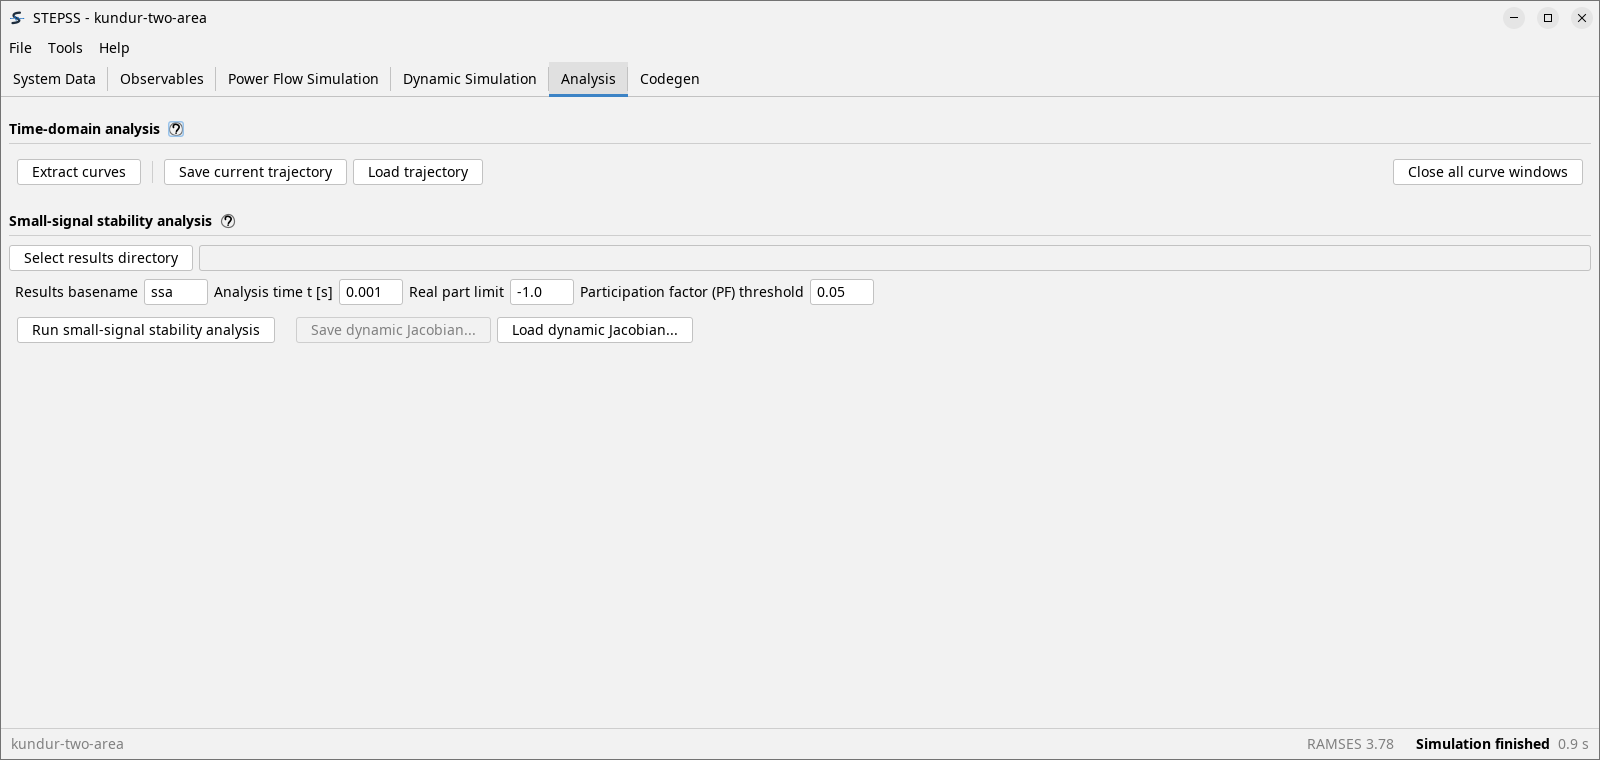
\includegraphics[width=0.98\linewidth]{figures/gui-analysis-light}
\caption{The Analysis tab with a completed run available.}
\end{figure}

The unlabelled field beside \textbf{Select results directory} is where results are
written, and it defaults to the working directory. The picker that \textbf{Extract
curves} opens, and the small-signal results window, are both shown on the pages
linked above.

\section{Codegen}\label{gui-interface:codegen}

Where a model of your own becomes part of the simulator, in the order the buttons
run:

\begin{small}\begin{longtable}[]{@{}
  >{\raggedright\arraybackslash}p{(\linewidth - 4\tabcolsep) * \real{0.3387}}
  >{\raggedright\arraybackslash}p{(\linewidth - 4\tabcolsep) * \real{0.6613}}
@{}}
\toprule\noalign{}
\begin{minipage}[b]{\linewidth}\raggedright
Button
\end{minipage} & \begin{minipage}[b]{\linewidth}\raggedright
What it does
\end{minipage} \\
\midrule\noalign{}
\endhead
\bottomrule\noalign{}
\endlastfoot
\textbf{Load files for Codegen} & Takes one or more model descriptions in the \hyperref[ch-user_models]{CODEGEN language} \\
\textbf{Run Codegen} & Translates them into Fortran, reporting each block with its equation and state counts \\
\textbf{Display loaded files} & Lists the Fortran files generated so far, not the descriptions that were read \\
\textbf{Save converted files} & Writes the generated \texttt{.f90} out \\
\textbf{Compile} & Builds and links it against the engine, giving a custom simulator \\
\textbf{Save executable} & Keeps that simulator, rather than rebuilding it next time \\
\end{longtable}\end{small}

Each enables as the previous step makes it meaningful. Once a custom simulator
exists, simulations run on it rather than on the bundled engine.

\begin{figure}[htbp]
\centering
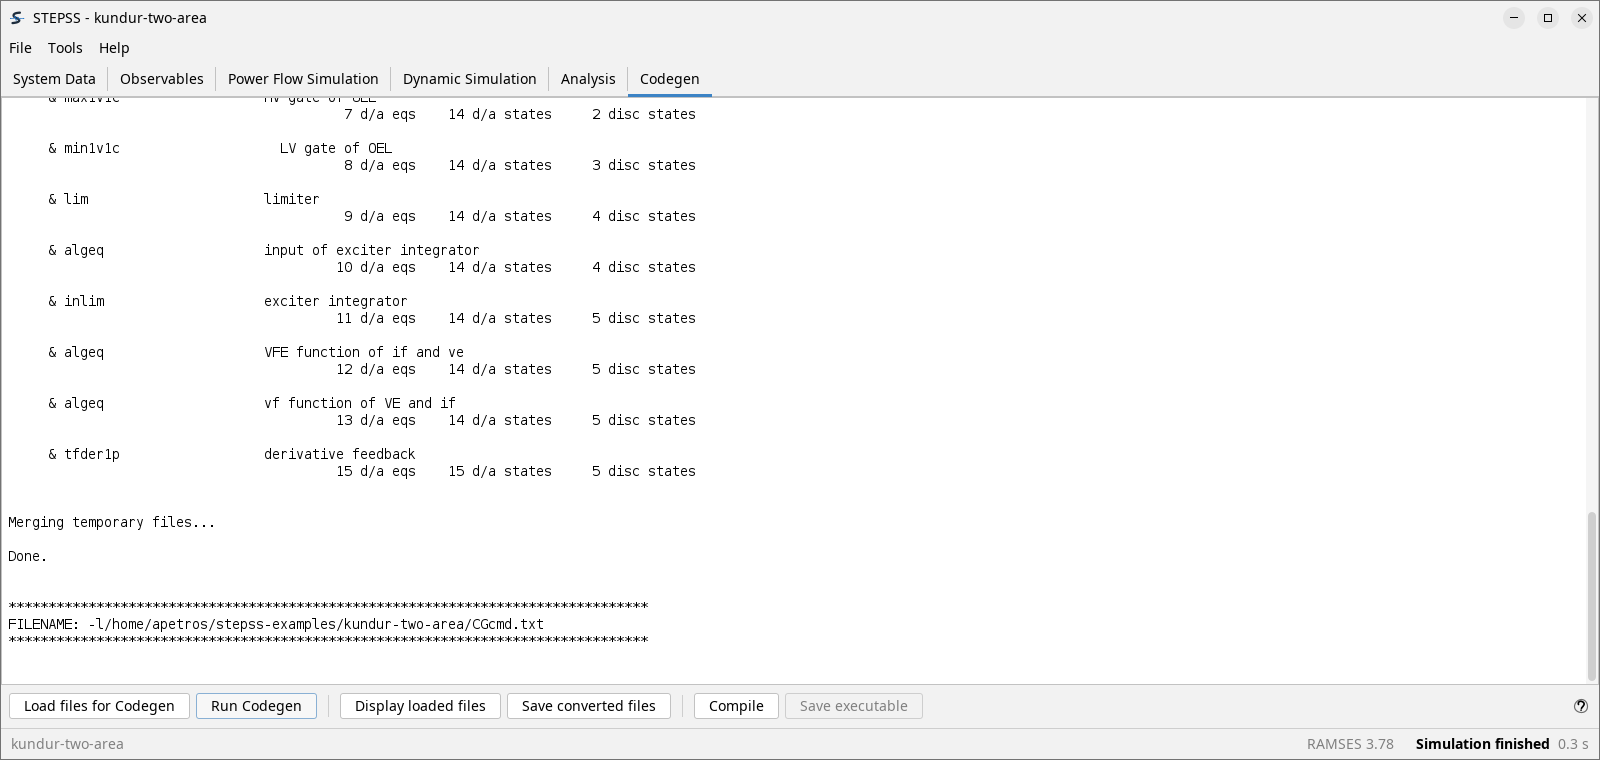
\includegraphics[width=0.98\linewidth]{figures/gui-codegen-light}
\caption{The Codegen tab after running CODEGEN on an IEEE AC1A exciter description.}
\end{figure}

Compiling needs a Fortran toolchain on the machine, which is
\hyperref[ch-install]{its own installation step};
translating a model does not.

\hyperref[ch-user_models]{User-Defined Models} is the reference for the model
language, and \hyperref[doc:cg-studio]{CODEGEN Studio} assembles models visually
instead of by hand.

\section{The menus}\label{gui-interface:the-menus}

\textbf{File} holds \textbf{Save configuration} and \textbf{Load configuration}, plus \textbf{Open
Examples} and \textbf{Exit}.

\begin{figure}[htbp]
\centering
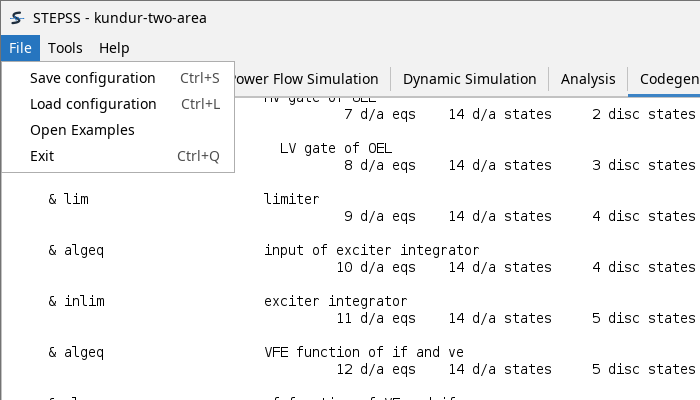
\includegraphics[width=0.98\linewidth]{figures/gui-file-menu-light}
\caption{The File menu open, holding Save configuration with Ctrl+S, Load configuration with Ctrl+L, Open Examples, and Exit with Ctrl+Q.}
\end{figure}

\textbf{Save configuration} writes a \texttt{.cfg} holding everything a run is made of: the
ten system data rows, the disturbance and observables files, the three runtime
observable rows, and the four recording checkboxes. \textbf{Load configuration} puts
them back, so a case set up once can be reopened and run in two clicks. A path
inside the \texttt{.cfg}'s own folder is stored relative to it, which means the folder
can be moved, copied or sent to a colleague whole; anything outside that folder
is stored as an absolute path and stays tied to the machine that saved it.

Two things the file does not carry. The observable dialog's five picker lists
are not saved, so a configuration saved with \textbf{Show observable dialog} ticked
says so when it loads and the lists need filling in again. And \texttt{.cfg} files
written by STEPSS releases before this format are refused rather than loaded:
they hold absolute paths belonging to whoever last saved them, so what they
name almost never exists on the machine opening them. Set the case up and save
it again.

\textbf{Tools} holds, in order, \textbf{Save command file} and \textbf{Save observables file},
which write out the files a command-line run needs; \textbf{Open in editor} and
\textbf{Select external simulator}; the working-directory controls \textbf{Select working
directory}, \textbf{Open working folder} and \textbf{Open terminal in working folder};
\textbf{Close all curve windows}; and, below a separator, the \textbf{Dark theme} toggle
and \textbf{Check for updates at startup}. The last two are ticks rather than
actions, and both are remembered between sessions.

\begin{figure}[htbp]
\centering
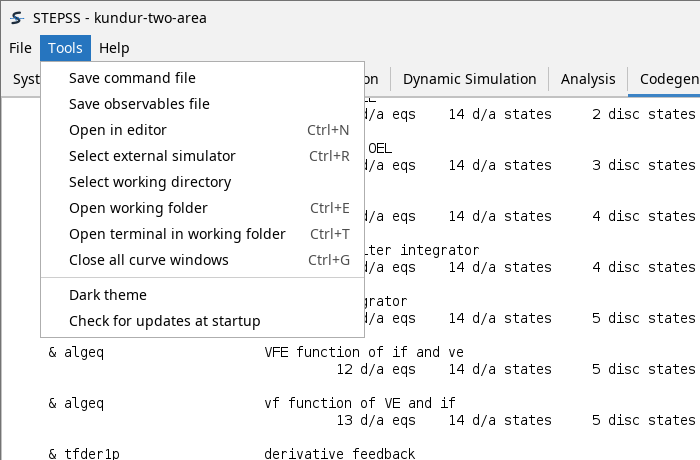
\includegraphics[width=0.98\linewidth]{figures/gui-tools-menu-light}
\caption{The Tools menu open, holding Save command file, Save observables file, Open in editor with Ctrl+N, Select external simulator with Ctrl+R, Select working directory, Open working folder with Ctrl+E, Open terminal in working folder with Ctrl+T and Close all curve windows with Ctrl+G, then below a separator the Dark theme and Check for updates at startup ticks, both unticked.}
\end{figure}

\textbf{Save command file} writes out the file the engine reads, listing the data,
disturbance, trajectory and observables files of the case in the order it
expects. It is what a run is made of, in one file.
\hyperref[doc:quickstart]{Quick Start} compares the two ways to drive the
engines.

\section{The status bar}\label{gui-interface:the-status-bar}

The working directory on the left; on the right the engine version and what the
application is doing. That last field runs from \textbf{Idle} through \textbf{Solving power
flow} to \textbf{Power flow finished} and \textbf{Simulation finished}, each with the
elapsed time, which is the quickest confirmation that a run actually did
something.

\begin{figure}[htbp]
\centering

\includegraphics[width=0.85\linewidth]{figures/gui-status-bar-light}
\caption{The status bar across the foot of the window: the working directory kundur-two-area on the left, and on the right the engine version RAMSES 3.78 followed by Simulation finished and an elapsed time of 0.9 seconds.}
\end{figure}
